\documentclass[12pt]{article}
\usepackage{rocca-homework}

\begin{document}

\title{MAT 304 Homework 1}
\date{\today}
\author{Lucas Vas}

\maketitle

\begin{problem}{Section 2.4 - Problem 28}
The logical form of part A is:

\begin{equation*}
	(P \wedge Q) \vee (P \wedge \sim Q) \vee (\sim P \wedge \sim Q)
\end{equation*}

The logical form of part B is:

\begin{equation*}
	(P \vee \sim Q)
\end{equation*}

When used with a truth table, the two logical forms are equivalent. The truth table is shown below:

\begin{center}
	\begin{tabular}{| c c | c | c |}
		\hline
		$P$ & $Q$ & $(P \wedge Q) \vee (P \wedge \sim Q) \vee (\sim P \wedge \sim Q)$ & $(P \vee \sim Q)$ \\
		\hline
		T   & T   & T                                                                 & T                 \\
		T   & F   & T                                                                 & T                 \\
		F   & T   & F                                                                 & F                 \\
		F   & F   & T                                                                 & T                 \\
		\hline
	\end{tabular}
\end{center}

Therefore, the two circuits shown in the original image are equivalent.

\end{problem}

\begin{problem}{Section 2.4 - Problem 31}
The circuit that represents the logical expression $(\sim P \wedge \sim Q) \vee (\sim P \wedge Q) \vee (P \wedge \sim Q)$ is:
\begin{center}
	%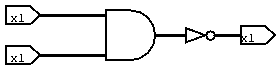
\includegraphics[width=8cm]{mat304-2.4-31.png}
	% Important: If latex complains about unicode characters,
% please use "\usepackage[utf8x]{inputenc}" in your preamble
% You can change the size of the picture by putting it into the construct:
% 1) \resizebox{10cm}{!}{"below picture"} to scale horizontally to 10 cm
% 2) \resizebox{!}{15cm}{"below picture"} to scale vertically to 15 cm
% 3) \resizebox{10cm}{15cm}{"below picture"} a combination of above two
% It is not recomended to use the scale option of the tikzpicture environment.
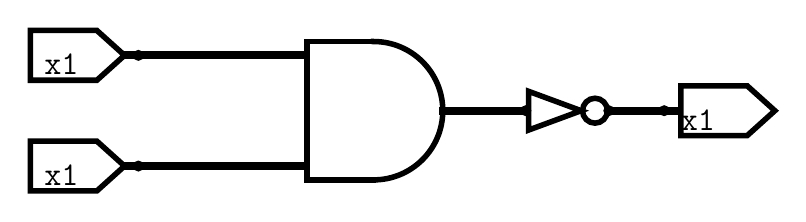
\begin{tikzpicture}[x=1pt,y=-1pt,line cap=rect]
	\def\logisimfontA#1{\fontfamily{cmr}{#1}} % Replaced by logisim, original font was "SansSerif"
	\def\logisimfontB#1{\fontfamily{cmtt}{#1}} % Replaced by logisim, original font was "Monospaced"
	\definecolor{custcol_0_0_0}{RGB}{0, 0, 0}
	\definecolor{custcol_ff_ff_ff}{RGB}{255, 255, 255}
	\draw [line width=3.0pt, custcol_0_0_0 ]  (215.0,35.0) -- (235.0,35.0) ;
	\draw [line width=3.0pt, custcol_0_0_0 ]  (155.0,35.0) -- (185.0,35.0) ;
	\draw [line width=2.0pt, custcol_0_0_0 ]  (205.0,35.0) -- (186.0,28.0) -- (186.0,42.0) -- cycle;
	\draw [line width=2.0pt, custcol_0_0_0]  (210.0,35.0) ellipse (4.5 and 4.5 );
	\fill [line width=2.0pt, custcol_0_0_0]  (215.0,35.0) ellipse (2.0 and 2.0 );
	\fill [line width=2.0pt, custcol_0_0_0]  (185.0,35.0) ellipse (2.0 and 2.0 );
	\draw [line width=2.0pt, custcol_0_0_0] (130.0,60.0) arc (90.0:-90.0:25.0 and 25.0 );
	\draw [line width=2.0pt, custcol_0_0_0 ]  (130.0,10.0) -- (106.0,10.0) -- (106.0,60.0) -- (130.0,60.0) ;
	\draw [line width=3.0pt, custcol_0_0_0 ]  (239.0,35.0) -- (236.0,35.0) ;
	\draw [line width=2.0pt, custcol_0_0_0 ]  (265.0,26.0) -- (275.0,35.0) -- (265.0,44.0) -- (241.0,44.0) -- (241.0,26.0) -- cycle;
	\logisimfontB{\fontsize{12pt}{12pt}\selectfont\node[inner sep=0, outer sep=0, custcol_0_0_0, anchor=base west] at  (241.0,42.0)  {x1};}
	\fill [line width=2.0pt, custcol_0_0_0]  (235.0,35.0) ellipse (2.0 and 2.0 );
	\draw [line width=3.0pt, custcol_0_0_0 ]  (40.0,15.0) -- (45.0,15.0) -- (105.0,15.0) ;
	\draw [line width=2.0pt, custcol_0_0_0 ]  (30.0,24.0) -- (40.0,15.0) -- (30.0,6.0) -- (6.0,6.0) -- (6.0,24.0) -- cycle;
	\logisimfontB{\fontsize{12pt}{12pt}\selectfont\node[inner sep=0, outer sep=0, custcol_0_0_0, anchor=base west] at  (11.0,22.0)  {x1};}
	\fill [line width=2.0pt, custcol_0_0_0]  (45.0,15.0) ellipse (2.0 and 2.0 );
	\draw [line width=3.0pt, custcol_0_0_0 ]  (40.0,55.0) -- (45.0,55.0) -- (105.0,55.0) ;
	\draw [line width=2.0pt, custcol_0_0_0 ]  (30.0,64.0) -- (40.0,55.0) -- (30.0,46.0) -- (6.0,46.0) -- (6.0,64.0) -- cycle;
	\logisimfontB{\fontsize{12pt}{12pt}\selectfont\node[inner sep=0, outer sep=0, custcol_0_0_0, anchor=base west] at  (11.0,62.0)  {x1};}
	\fill [line width=2.0pt, custcol_0_0_0]  (45.0,55.0) ellipse (2.0 and 2.0 );
\end{tikzpicture}

\end{center}
\end{problem}

\begin{problem}{Section 3.4 - Problem 20}
The argument `All dogs are carnivorous, and Aaron is not a dog, therefore Aaron is not carnivorous' is invalid.
This is an example of the inverse error. If we create a truth table for the argument, we can see that the argument is invalid:

\begin{center}
	\begin{tabular}{| c c | c |}
		\hline
		$P$ & $Q$ & $P \rightarrow Q$ \\
		\hline
		T   & T   & T                 \\
		T   & F   & F                 \\
		F   & T   & T                 \\
		F   & F   & T                 \\
		\hline
	\end{tabular}
\end{center}

This specific case where Aaron is not a dog falls in multiple cases where the argument is valid - one where he is carnivorous and one where he is not.
Therefore, the argument is invalid, even though Aaron is not a dog and he may not be carnivorous.

For the second part of this problem, which generalizes the statement, we can see that the argument is still invalid. The truth table will be the same,
and the reasoning for the invalidity of the argument will still hold.
\end{problem}

\begin{problem}{Section 3.4 - Problem 22}
The argument given can be simplified to the following logical form:
\begin{equation*}
	\begin{split}
		S(x) \rightarrow V(x) \\
		T(x) \rightarrow V(x) \\
		\hline
		\therefore S(x) \wedge T(x)
	\end{split}
\end{equation*}

I do not believe that this is a valid argument - the premises, when combined, do not necessarily imply the conclusion.
When $S(x)$ is true, this does not immediately imply that $T(x)$ is true. The same goes for when $T(x)$ is true. Therefore,
the argument is invalid.
\end{problem}

\begin{problem}{Section 3.4 - Problem 27}
The argument given can be simplified to the following logical form:
\begin{equation*}
	\begin{split}
		I(x) \rightarrow \sim P(x) \\
		P(l)                       \\
		\hline
		\therefore \sim I(l)
	\end{split}
\end{equation*}

This is a perfect example of modus tollens. It is a valid argument.
\end{problem}

\end{document}
